\begin{figure} %[thpb]
	\centering
	%\shorthandoff{;} 
	\resizebox{\textwidth}{!}{%
		\begin{minipage}[b]{.5\linewidth}
			\centering
			\subcaptionbox{\label{subfig_coupling_effect_a}}
			{
				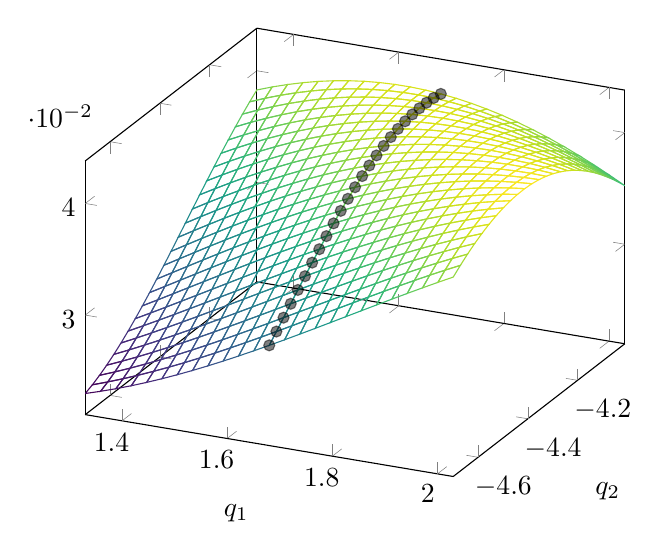
\begin{tikzpicture} [%
					declare function = {%
						xTerm(\x,\y) =  ((27*sin(deg(\x) + deg(\y)))/200 + (113*sin(deg(\x) + deg(\y) + deg(1497/1000)))/1000)^2 + ((27*sin(deg(\x) + deg(\y)))/200 + (113*sin(deg(\x) + deg(\y) + deg(1497/1000)))/1000 + (31*sin(deg(\x)))/200)^2 + (12769*sin(deg(\x) + deg(\y) + deg(1497/1000))^2)/1000000;
					}%
					]%
					\begin{axis}[%
					domain=1.33:2.03,
					y domain=-4.7:-4.01,
					xlabel={$ q_1 $},
					ylabel={$ q_2 $},
					colormap/viridis,
					%point meta min=-0.015, 
					%point meta max=0.042,
					%view={25}{40},
					]
					%
						\addplot3 [mesh] {xTerm(x,y)};
						\addplot3 [only marks, samples at={1.68}%, y samples at={-4.355}
						, opacity = 0.5] {xTerm(x,y)};
					\end{axis}
				\end{tikzpicture}
			}
		\end{minipage}
		\begin{minipage}[b]{.5\linewidth}
			\centering
			\subcaptionbox{\label{subfig_coupling_effect_b}}
			{
				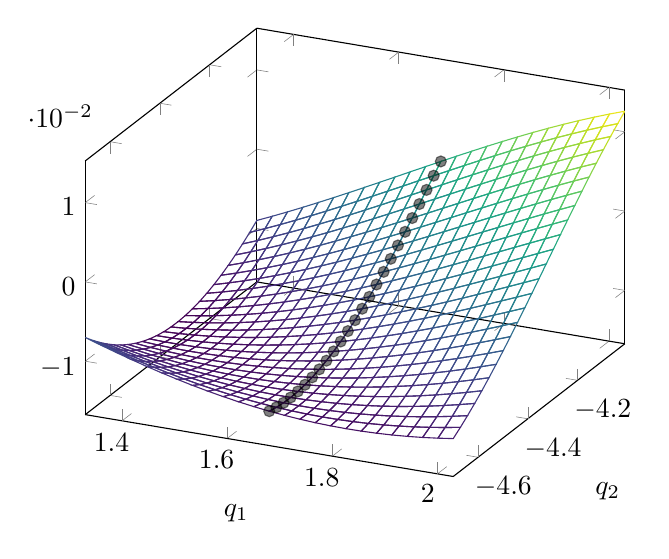
\begin{tikzpicture}  [%
				declare function = {%
					zTerm(\x,\y) =  -(961*sin(2*deg(\x)))/80000 - (729*sin(2*deg(\x) + 2*deg(\y)))/40000 - (38307*sin(2*deg(\x) + 2*deg(\y) + deg(1497/500)))/2000000 - (3051*sin(2*deg(\x) + 2*deg(\y) + deg(1497/1000)))/100000 - (837*sin(2*deg(\x) + deg(\y)))/40000 - (3503*sin(2*deg(\x) + deg(\y) + deg(1497/1000)))/200000;
				}%
				]%
				\begin{axis}[%
				domain=1.33:2.03,
				y domain=-4.7:-4.01,
				xlabel={$ q_1 $},
				ylabel={$ q_2 $},
				colormap/viridis,
				%point meta min=-0.015, 
				%point meta max=0.042,
				%view={25}{40}, 
				]
				%
					\addplot3 [mesh] {zTerm(x,y)};
					\addplot3 [only marks, samples at={1.68}%, y samples at={-4.355}
					, opacity = 0.5] {zTerm(x,y)};
				\end{axis}
				\end{tikzpicture}
			}
		\end{minipage}
	}
	%\shorthandon{;} 
	\caption{Variations des termes matriciels de \cref{eq_coupling_effect_jacobian}, pour $ q_3 = 1.5 $. La position articulaire $ q_1 = 1.68 $ est signalée par des marqueurs circulaires. \cref{subfig_coupling_effect_a} Termes de la diagonale influençant la position en $ x $, \cref{subfig_coupling_effect_b} termes de couplages en $ x $ qui sont multipliés par  $ f_z $. Les positions articulaires sont données en radians.}
		%Variation of terms from matrix \cref{eq_coupling_effect_jacobian}, for $ q_3 = 1.5 $, $ q_1 = 1.68 $ is notified by the circular black markers (a) Diagonal term on $ x $, (b) Coupling term on $ x $ multiplied by $ f_z $. Joint values are provided in radians.}
	\label{fig_coupling_effect_joint_ctrl}
\end{figure}

% 